\input{header_slides.tex}

\begin{document}

\title[Dynamics of Urban Systems]{Empowering Urban Governance through Urban Science: Multi-Scale Dynamics of Urban Systems Worldwide}
\author[Raimbault, Denis and Pumain]{J.~Raimbault$^{1,2,3\ast}$, E. Denis$^3$ and D.Pumain$^3$\\
\texttt{j.raimbault@ucl.ac.uk}
}


\institute[CASA, UCL]{$^{1}$CASA, UCL\\
$^{2}$UPS CNRS 3611 Complex Systems Institute Paris\\
$^{3}$UMR CNRS 8504 G{\'e}ographie-cit{\'e}s
}


\date[December 7th 2020]{ISWEE 2020\\
Session 2: Sustainable Cities and Society\\
December 7th 2020
}

\frame{\maketitle}

% 

%Abstract:	Cities are facing many sustainability issues in the context of the current global interdependency characterized by an economic uncertainty coupled to climate changes, which challenge their local policies aiming to better conciliate reasonable growth with livable urban environment. The urban dynamic models developed by the so-called “urban science” can provide a useful foundation for more sustainable urban policies. It implies that their proposals have been validated by correct observations of the diversity of situations in the world. However, international comparisons of the evolution of cities often produce unclear results because national territorial frameworks are not always in strict correspondence with the dynamics of urban systems. We propose to provide various compositions of systems of cities in order to better take into account the dynamic networking of cities that go beyond regional and national territorial boundaries. Different models conceived for explaining city size and urban growth distributions enable the establishing of a correspondence between urban trajectories when observed at the level of cities and systems of cities. We test the validity and representativeness of several dynamic models of complex urban systems and their variations across regions of the world, at the macroscopic scale of systems of cities. The originality of the approach resides in the way it considers spatial interaction and evolutionary path dependence as major features in the general behavior of urban entities. The models studied include diverse and complementary processes, such as economic exchanges, diffusion of innovations, and physical network flows. Complex systems dynamics is in principle unpredictable, but contextualizing it regarding demographic, income, and resource components may help in minimizing the forecasting errors. We use, among others, a new unique source correlating population and built-up footprint at world scale: the Global Human Settlement built-up areas (GHS-BU). Following the methodology and results already obtained in the European GeoDiverCity project, including USA, Europe, and BRICS countries, we complete them with this new dataset at world scale and different models. This research helps in further empirical testing of the hypotheses of the evolutionary theory of urban systems and partially revising them. We also suggest research directions towards the coupling of these models into a multi-scale model of urban growth.


\section{Introduction}


\sframe{How to explain urban growth?}{

\begin{itemize}
	\item Apparent direct \textbf{causes} : intentions/actions from urban actors (policies, locational strategies from firms, residential migrations \ldots)
	\item But \textbf{statistical observation} (thousands of cities, over centuries) : each city has a probability of growing similar to other cities belonging to the same territorial system	
\end{itemize}

\medskip
$\rightarrow$ ``distributed growth'' on the long run with many local and temporal fluctuations

}


\sframe{Gibrat's model}{

``Proportional'' growth = growth rates are equiprobable for any city size and not correlated with previous rate

\medskip

Good fit $\rightarrow$ double explanatory gain: 

\begin{itemize}
	\item Persistency of urban spatial patterns and hierarchies
	\item The statistical shape of urban sizes distribution (Zipf’s law or lognormal) as generated from growth process
\end{itemize}

\cite{gibrat1931inegalits} \cite{robson1973urban} \cite{pumain1982dynamique}


}


\sframe{Gibrat’s model}{
%
\textit{A satisfying proxy but some empirical contradiction}
%
\bigskip
%
\begin{enumerate}
\item The observed distributions of city sizes (actually: settlement sizes including hamlets, villages, towns and SMAs) are lognormal (evidence from \cite{robson1973urban}, \cite{pumain1982dynamique}, \cite{eeckhout2004gibrat}, \cite{decker2007global})
\item Gibrat’s growth model leads to a lognormal distribution of city sizes
\item But Gibrat’s growth model hypothesis are rejected (correlation between growth rates and city size, correlation between successive growth rates)
\end{enumerate}

}
%
%\sframe{Evolutionary urban theory}{
%
%\textit{Innovation diffusion and spatial integration of urban systems}
%
%\bigskip
%
%\begin{itemize}
%\item In new urban systems, as in USA, there is a spatial filling process that occur through waves of urban growth (urban Frontier) corresponding to the diffusion of economic cycles
%\item In mature urban systems, like in France, the innovations diffusion reaches cities that are not spatially regularly arranged but already experienced other growth periods according to distinct cycles of urban specialisation
%\end{itemize}
%
%}
%
%
\sframe{Evolutionary urban theory and scaling laws}{

An \textbf{Evolutionary Urban Theory} linking scaling laws to a geographical model of urban growth with spatial interaction and innovation cycles \cite{pumain1997pour} \cite{pumain2018evolutionary}

\bigskip

\begin{itemize}
\item \cite{pumain2006evolutionary} suggest to replace a generic statistical model of growing independent entities (Gibrat’s urban growth model) by a model of spatially and temporally interdependent entities (i.e. the geographical concept of ``system of cities'' or ``settlement system'')
\item It reproduces the observations on differential scaling parameters for urban activities according to their age in innovation cycles \cite{favaro2011gibrat}
\item It also makes explicit the multilevel dynamics of interurban competition for capturing innovation, which may itself generate new innovation through interurban emulation, within an evolutionary perspective
\end{itemize}

}


\sframe{Testing the evolutionary urban theory}{

\footnotesize

\textit{How are stylized facts on systems of cities robust and general ?}

\medskip

$\rightarrow$ empirical study with the new Global Human Settlement layer dataset

\medskip

\textit{How can dynamical models of urban systems be applied in the context of the evolutionary urban theory ?}

\medskip

$\rightarrow$ test of six dynamical models, based on geographical interactions between cities but different dimensions, on different systems of cities and worldwide

%\medskip

\begin{center}
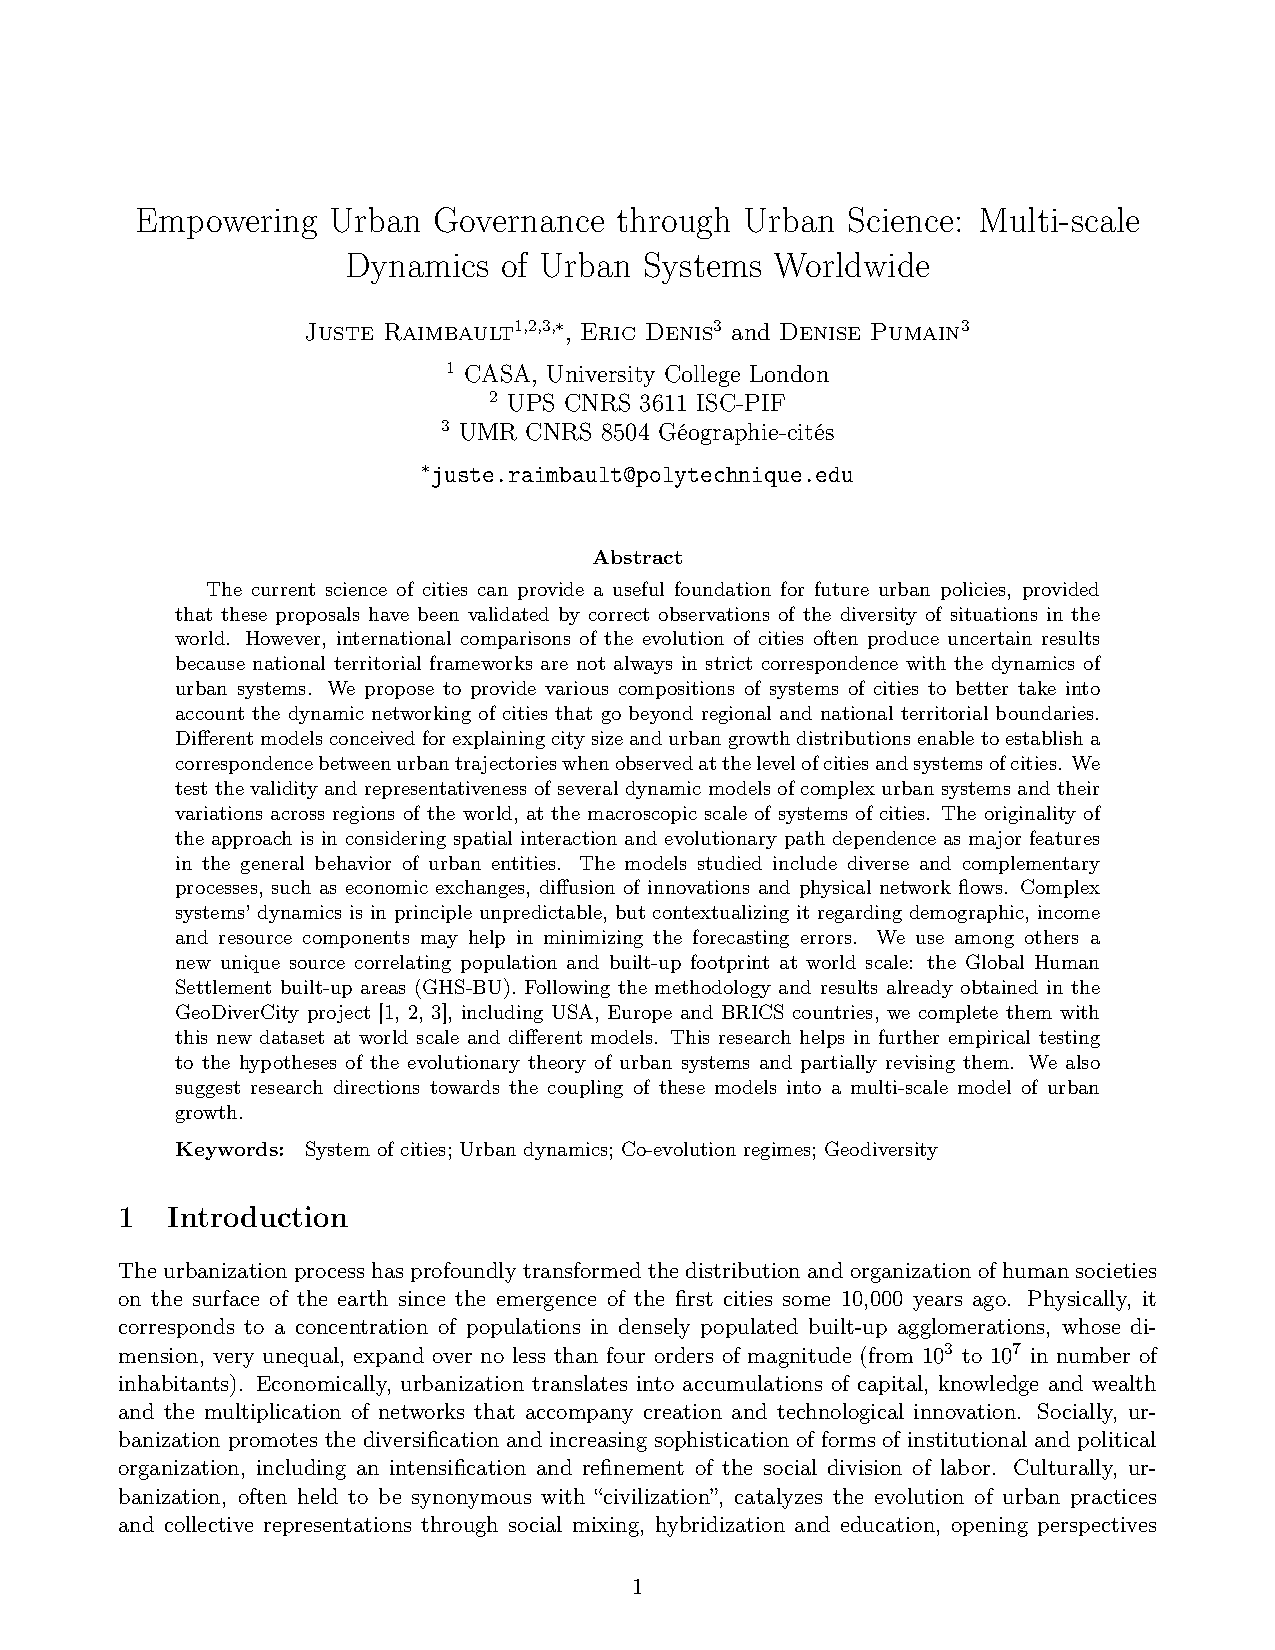
\includegraphics[width=0.77\textwidth]{figures/paper.png}
\end{center}


}


\section{Data analysis}


\sframe{A new source of data on global urbanization}{

\begin{itemize}
	\item GHSL (Global Human Settlement Layer) : GEO Human Planet Initiative (European Commission)
	\item Built up area from satellite images 40 m + population data 250 m $\rightarrow$ 1 km2 grid
	\item 13 000 urban areas > 50 000 inhab.
	\item Surface, population in 1975, 1990, 2000, 2015
	\item GDP, Green surfaces, Pollutants 1990-2015
\end{itemize}

}



% number of areas per country
% summary(countrycount$count)
%   Min. 1st Qu.  Median    Mean 3rd Qu.    Max. 
%   1.00    4.00   13.00   72.17   48.75 3248.00 


%
%\sframe{Population distributions}{
%
%\begin{center}
%    \includegraphics[width=0.7\textwidth]{figures/population_distributions.png}
%\end{center}
%
%\textit{Temporal stability of the shape of global population distribution}
%
%}


\sframe{Urban systems summary}{
    
    % \cite{pumain2015multilevel} : number of cities / urban pop for each urban system
    % Summary table : number of cities, rank size slope, primacy index, total population
    
    % summary - 2015 - geodivercity urban systems

    \textit{Summary statistics in 2015 for urban systems \cite{pumain2015multilevel}}
    
    \smallskip
    
%    {\tiny
%    \begin{center}
%    \begin{tabular}{|c|c|c|c|c|c|}
%    \hline
%        System & Population & Cities & Primacy & Rank-size & R2  \\\hline
%         Europe & 188Mio & 693 & 1.01 & $0.94 \pm 0.0026$ & 0.994  \\
%         China & 567.2Mio & 1850 & 1.66 & $0.91 \pm 0.0011$ & 0.997  \\
%         Brazil & 111.7Mio & 349 & 1.95 & $0.99 \pm 0.0026$ & 0.998  \\
%         India & 703.1Mio & 3248 & 1.22 & $0.78 \pm 0.0009$ & 0.996  \\
%         South Africa & 25.3Mio & 77 & 1.85 & $1.05 \pm 0.020$ & 0.974  \\
%         US & 153Mio & 324 & 1.12 & $1.16 \pm 0.0054$ & 0.992  \\
%         FSU & 120.3Mio & 450 & 3.27 & $0.92 \pm 0.0062$ & 0.979  \\\hline
%    \end{tabular}
%    \end{center}
%    }
{%\tiny
    \begin{center}
    \begin{tabular}{|c|c|c|c|c|c|}
    \hline
        System & Pop (M) & Pop geodiv. & Cities & Rank-size  \\\hline
         Europe & 188 & 291 & 693 & $0.94$  \\
         China & 567 & 481 & 1850 & $0.91$  \\
         Brazil & 112 & 161 & 349 & $0.99$  \\
         India & 703 & 427 & 3248 & $0.78$  \\
         South Africa & 25 & 25 & 77 & $1.05$ \\
         US & 153 & 324 & 287 & $1.16$  \\
         FSU & 120 & 174 & 450 & $0.92$ \\\hline
    \end{tabular}
    \end{center}
    }
    
    %\smallskip

	%\begin{center}
%		\includegraphics[height=0.4\textheight]{figures/geodivercity-summary.png}
%	\end{center}


}





\sframe{Urban systems hierarchy}{

Reproducing results of \cite{pumain2015multilevel} for large urban systems

% Brazil, China, US, Europe, South Africa, URSS, India

\begin{center}
    \includegraphics[width=0.53\textwidth,height=0.5\textheight]{../../../../Communications/2019/ECTQG2019/Communication/figures/RankSize_Europe-China-Brazil-India-SouthAfrica-UnitedStates-FormerSovietUnion_years-90-00-15.png}
    \includegraphics[width=0.45\textwidth]{../../../../Communications/2019/ECTQG2019/Communication/figures/geodivercity-ranksize.png}
\end{center}

\medskip

$\rightarrow$ \textbf{Robustness of qualitative stylized facts to the database}

}

\sframe{Rank-size by continents or trade areas}{

\begin{center}
    \includegraphics[width=0.48\textwidth]{../../../../Papers/EvolutionaryTheory/paper/figures/Fig1.png}
    \includegraphics[width=0.48\textwidth]{../../../../Papers/EvolutionaryTheory/paper/figures/Fig2.png}
\end{center}

\medskip

$\rightarrow$ \textbf{Possibility to extend analysis to other consistent geographical ensembles}

}



\sframe{Correlations between urban indicators}{

% includes test of gibrat law : correlation pops / growth rates

\begin{center}
    %\includegraphics[width=0.46\textwidth]{figures/correlations_00.png}\hspace{0.2cm}
    \includegraphics[width=0.7\textwidth]{../../../../Papers/EvolutionaryTheory/paper/figures/Fig3.png}
\end{center}

%\medskip

%$\rightarrow$ no apparent deviation to Gibrat's law with this dataset (importance of definition of cities in scaling laws \cite{cottineau2017diverse})


}


\sframe{Linking urban growth and built-up area growth}{

\begin{center}
\includegraphics[width=0.85\textwidth]{../../../../Papers/EvolutionaryTheory/paper/figures/Fig4.png}
\end{center}

\footnotesize

\textit{Geographical structure in the relation between population growth and built-up area growth}

}

%
%\sframe{Scaling laws}{
%
%%reproduction / Generalizing existing studies
%
%\begin{center}
%%    \includegraphics[width=0.32\textwidth]{figures/Built-fitted_Europe-China-Brazil-India-SouthAfrica-UnitedStates-FormerSovietUnion_years-90-00-15.png}
%    \includegraphics[width=0.48\textwidth]{figures/GDP-fitted_Europe-China-Brazil-India-SouthAfrica-UnitedStates-FormerSovietUnion_years-90-00-15.png}
%    \includegraphics[width=0.48\textwidth]{figures/Emissions-fitted_Europe-China-Brazil-India-SouthAfrica-UnitedStates-FormerSovietUnion_years-90-00-15.png}
%\end{center}
%
%}

\sframe{Evolution of scaling exponents}{

% evolution of scaling exponents in time





\begin{center}
    %\includegraphics[width=0.32\textwidth,height=0.45\textheight]{figures/Built-evolution_Europe-China-Brazil-India-SouthAfrica-UnitedStates-FormerSovietUnion_years-90-00-15.png}
    \includegraphics[width=0.48\textwidth,height=0.45\textheight]{../../../../Communications/2019/ECTQG2019/Communication/figures/Emissions-evolution_Europe-China-Brazil-India-SouthAfrica-UnitedStates-FormerSovietUnion_years-90-00-15.png}
    \includegraphics[width=0.48\textwidth,height=0.45\textheight]{../../../../Communications/2019/ECTQG2019/Communication/figures/GDP-evolution_Europe-China-Brazil-India-SouthAfrica-UnitedStates-FormerSovietUnion_years-90-00-15.png}
\end{center}

\medskip

\textit{All indicators are stable in their confidence range}

}


\sframe{Summary of scaling exponents}{


\begin{center}
\small
    \begin{tabular}{|c|c|c|c|c|c|}
    \hline
    System & Built-up area & GDP & Emissions \\\hline
Europe & $0.93 \pm 0.016$ (0.83) & $1.15 \pm 0.019$ (0.83) & $1.50 \pm 0.038$ (0.69) \\
China & $1.06 \pm 0.019$ (0.62)  & $1.14 \pm 0.011$ (0.85)  & $1.84 \pm 0.037$ (0.57) \\
Brazil & $0.98 \pm 0.025$ (0.81)  & $1.10 \pm 0.055 $ (0.54) & $1.71 \pm 0.053$ (0.75) \\
India & $1.34 \pm 0.031$ (0.36) & $1.25 \pm 0.022$ (0.50) & $1.54 \pm 0.031$ (0.42) \\
S. Africa & $1.18 \pm 0.090$ (0.69) & $1.08 \pm 0.028$ (0.95) & $1.56 \pm 0.087$  (0.81) \\
US & $0.97 \pm 0.015$ (0.92) & $1.04 \pm 0.069$ (0.99) &$ 1.34 \pm 0.03$ (0.84) \\
FSU & $0.97 \pm 0.035$ (0.63) & $1.17 \pm 0.041$ (0.65) & $1.95 \pm 0.088$ (0.52)\\\hline
\end{tabular}
\end{center}

\bigskip

$\rightarrow$ more general, more or less consistent study of scaling (``basic'' indicators but on consistent and global geographical areas)
% vs shitty on number of cinemas etc - we do not really care.

}



%\sframe{Fitting scaling laws}{

% \cite{finance2018absent}
% \cite{clauset2009power}
% \cite{leitao2016scaling}
% \cite{broido2019scale}
% \cite{smith2019biochemical}

% summary table of Goodness of fit for - classical scaling, with cutoff, as piecewise linear

%\textit{Alternative models for better fit of scaling laws}

% test alternative scaling models ?

%}


\section{Dynamical models}

\sframe{Dynamical models of urban growth}{

\textit{Testing interaction-based dynamical models for urban growth}

\bigskip

\begin{itemize}
	\item The Favaro-Pumain model for the diffusion of innovation \cite{favaro2011gibrat}
	\item The Marius model family based on economic exchanges \cite{cottineau2014evolution}
	\item An interaction model including physical transportation networks \cite{raimbault2018indirect}
\end{itemize}


}



\sframe{Description of models}{

% increasing complexity for the presentation of models

\begin{columns}
	\begin{column}{0.33\textwidth}
		\textbf{Network interaction model}
		
		\medskip

		\begin{itemize}
			\item Endogenous growth
			\item Interactions inducing growth through gravity potential
			\item Static physical network taken into account (geographical shortest path with topography)
		\end{itemize}
		
	\end{column}
	\vrule{}
	\begin{column}{0.33\textwidth}
		%\vspace{-1cm}
		\textbf{Favaro-Pumain model}
		
		\medskip
		
		\begin{itemize}
			\item Endogenous growth
			\item Innovation emerge and diffuse in cities
			\item Growth rates adapted according to utility of innovation and level of adaptation
		\end{itemize}
			
	\end{column}
	\vrule{}
	\begin{column}{0.33\textwidth}
		\textbf{Marius model}
		
		\medskip
		
		\begin{itemize}
			\item Cities produce economic goods
			\item Economic exchanges are estimated according to gravity flows
			\item Populations grow depending on final economic balances
		\end{itemize}

		
	\end{column}
\end{columns}



}


\sframe{Implementation and experiments}{

%\footnotesize
\justify

\textbf{Implementation}

Models implemented in \texttt{scala}, using the \texttt{spatialdata} library 

\cite{raimbault2020scala}

\url{https://github.com/openmole/spatialdata}



\bigskip

\textbf{Model exploration and validation}

Integrated seamlessly into the OpenMOLE workflow engine

\cite{reuillon2013openmole} for model exploration, sensitivity analysis and validation

\url{https://openmole.org/}

\begin{center}
\includegraphics[width=0.1\linewidth]{figures/iconOM.png}
\includegraphics[width=0.4\linewidth]{figures/openmole.png}
\end{center}



}





\sframe{Calibration of dynamical models}{

\includegraphics[width=\textwidth]{../../../../Papers/EvolutionaryTheory/paper/figures/Fig5.png}

}


\sframe{Indian urban system: direct interactions}{

% systems on which the behavior is particularly interesting ?

\centering
\includegraphics[width=0.85\textwidth]{../../../../Papers/EvolutionaryTheory/paper/figures/Fig6.png}

}


\sframe{Brazilian urban system: multiple factors}{

\centering
\includegraphics[width=0.9\textwidth,height=0.8\textheight]{../../../../Papers/EvolutionaryTheory/paper/figures/Fig7.png}

\footnotesize
\textit{Importance of topography; innovation processes mostly.}

}

\sframe{China: similar models}{

\centering
\includegraphics[width=0.9\textwidth,height=0.8\textheight]{../../../../Papers/EvolutionaryTheory/paper/figures/Fig8.png}

\footnotesize
\textit{No clear best model: other processes in play ? (strong top-down planning)}

}



\sframe{Worldwide calibration of models}{

% new results with the worldwide run

\centering

\includegraphics[height=0.9\textheight]{../../../../Papers/EvolutionaryTheory/paper/figures/Fig9.png}

}

\section{Discussion}

\sframe{Towards multi-scale models}{

\justify

\textit{Crucial aspect of processes at multiple scales and feedback between these \cite{pumain2008socio}; need to be taken into account to build sustainable territorial policies \cite{rozenblat2018conclusion}}

\bigskip

$\rightarrow$ Empirical analysis of contradictory sustainability indicators on endogenous European mega-city regions \cite{raimbault2019multi}

\medskip

$\rightarrow$ A parsimonious multi-scalar urban growth model coupling spatial interactions \cite{raimbault2020indirect} at the macroscopic scale with reaction-diffusion models for urban form \cite{raimbault2018calibration} at the mesoscopic scale in \cite{raimbault:halshs-02351722}

\medskip

$\rightarrow$ A co-evolution model between cities and networks including physical transportation network \cite{raimbault2020hierarchy} (extended with governance processes - \textit{forthcoming talk this Wednesday at CCS2020})


}

\sframe{Discussion}{


% - robustesse des faits stylises / des conclusions theoriques 
% - complementarite
% - historique/politique - dependance au chemin ! pas inertie - adaptation aux contextes changeants - renforcement des hierarchies - temps tres long


\textbf{Synthesis}

$\rightarrow$ robustness of stylized facts, and of theoretical constructions

$\rightarrow$ complementarity of processes and models

$\rightarrow$ importance of the historical/political/geographical context, path-dependency


\medskip

\textbf{Open questions:}

$\rightarrow$ linking urban scaling and dynamical models

$\rightarrow$ endogenous consistent urban systems

$\rightarrow$ multiscale models

% applicable knowledge

\medskip

\textbf{Applications}

$\rightarrow$ Statistical predictability of city growth and size on short time periods

%$\rightarrow$ Largest metropolises are not ``monstruopolises''

$\rightarrow$ Transfer to practitioners: proactive adaptive strategies are necessary (imitation, or anticipation and risk), emulation (co-opetition)

$\rightarrow$ Robustness, variation and sustainability of urban systems (neither norm nor optimum)

}



\sframe{Conclusion}{


\justify

\vspace{-1cm}

$\rightarrow$ Robustness of results regarding data sources, multiple models. \textbf{Need for more systematic model exploration and sensitivity analysis.}

\smallskip

$\rightarrow$ Model complementarity. \textbf{Need for more integrated models.}

\smallskip

$\rightarrow$ Multiple perspectives on urban systems? \textbf{Need for more interdisciplinarity.}

\bigskip

%\footnotesize


\smallskip

\textbf{Open repository} for models and results at

\url{https://github.com/JusteRaimbault/UrbanGrowth}

\url{https://github.com/openmole/spatialdata}

\bigskip

\textbf{Paper} (open access) at \url{https://doi.org/10.3390/su12155954}

\bigskip

\textbf{Acknowledgments}: thanks to the \textit{European Grid Infrastructure} for access to the infrastructure.


}






\sframe{Reserve slides}{

\centering

\Large

\textbf{Reserve Slides}

}




\sframe{Rank-size by continents or trade areas}{

 \begin{center}
    \begin{tabular}{|c|c|c|c|c|c|}
    \hline
    System & Population & Cities & Primacy & Rank-size & R2  \\\hline
Europe & 288Mio & 1067 & 1.45 & $0.93 \pm 0.003$  & 0.991 \\
America & 547Mio & 1521 & 1.02 & $1.02 \pm 0.002$ & 0.996 \\
Asia & 2143Mio & 7737 & 1.12 & $ 0.87 \pm 0.0004$ & 0.998 \\
Africa & 585Mio & 2876 & 1.70 & $0.78 \pm 0.0008$ & 0.997 \\
Oceania & 19Mio & 86 & 1.08 & $0.91 \pm 0.027$ & 0.926\\\hline
\end{tabular}
    \end{center}
    
    \medskip
    
    \begin{center}
    \begin{tabular}{|c|c|c|c|c|c|}
    \hline
    System & Population & Cities & Primacy & Rank-size & R2  \\\hline
ASEAN & 293Mio & 874 & 1.67 & $0.92 \pm 0.003$ & 0.993 \\
MERCOSUR & 220Mio & 657 & 1.37 & $1.00 \pm 0.0016$ & 0.998 \\
COMESA & 252Mio & 1367 & 3.39 & $0.72 \pm 0.0014$ & 0.995 \\
EEA & 194Mio & 720 & 1.01 & $0.94 \pm 0.0026$ & 0.994 \\ \hline
\end{tabular}
    \end{center}

\medskip

$\rightarrow$ similar qualitative patterns, but different thematic questions can be tackled

}





\sframe{Scaling by continents or trade areas}{

\footnotesize

\begin{center}
    \begin{tabular}{|c|c|c|c|c|c|}
    \hline
    System & Built-up area & GDP & Emissions \\\hline
Europe & $0.93 \pm 0.016$ (0.76) & $1.12 \pm 0.024$ (0.67) & $1.58 \pm 0.039$ (0.61) \\
America & $1.11 \pm 0.030$ (0.48) & $1.23 \pm 0.027$ (0.57) & $1.69 \pm 0.041$  (0.53) \\
Asia & $1.32 \pm 0.022$ (0.32) & $1.30 \pm 0.016$ (0.47) & $1.78 \pm 0.024$ (0.42) \\
Africa & $1.57 \pm 0.049$ (0.26) & $1.45 \pm 0.043$ (0.29) & $2.04 \pm 0.054$ (0.33) \\
Oceania & $2.56 \pm 0.44$ (0.28) & $1.95 \pm 0.32$ (0.33) & $2.97 \pm 0.44$ (0.34) \\\hline
\end{tabular}
\end{center}

\medskip

\begin{center}
    \begin{tabular}{|c|c|c|c|c|c|}
    \hline
    System & Built-up area & GDP & Emissions \\\hline
ASEAN & $1.26 \pm 0.049$ (0.43) & $1.23 \pm 0.041$ (0.51) & $1.75 \pm 0.067$ (0.44) \\
MERCOSUR & $1.04 \pm 0.040$ (0.50) & $1.15 \pm 0.035$ (0.62) & $1.72 \pm 0.050$ (0.64) \\
COMESA & $1.65 \pm 0.074$ (0.26) & $1.52 \pm 0.072$ (0.26) & $1.93 \pm 0.085$ (0.28) \\
EEA & $0.93 \pm 0.015$ (0.84) & $1.15 \pm 0.019$ (0.83) & $1.50 \pm 0.037$ (0.69)\\\hline
\end{tabular}
\end{center}

}





\sframe{Models settings}{

$\rightarrow$ Work under Gibrat independence assumptions, i.e. $\Covb{P_i\left(t\right)}{P_j\left(t\right)} \textrm{=}0$. If $\vec{P}\left(t\textrm{+}1\right)\textrm{=}\mathbf{R}\cdot \vec{P}\left(t\right)$ where $\mathbf{R}$ is also independent, then $\Eb{\vec{P}\left(t\textrm{+}1\right)}\textrm{=}\Eb{\mathbf{R}}\cdot\Eb{\vec{P}}\left(t\right)$. Consider expectancies only (higher moments computable similarly)

\medskip

$\rightarrow$ With $\vec{\mu}\left(t\right)\textrm{=}\Eb{\vec{P}\left(t\right)}$, we generalize this approach by taking $\vec{\mu}\left(t\textrm{+}1\right)=f\left(\vec{\mu}\left(t\right)\right)$

}



\sframe{Network model}{

Direct network interaction model \cite{raimbault2018indirect}:

\medskip

Let $\vec{\mu}\left(t\right)\textrm{=}\Eb{\vec{P}\left(t\right)}$ cities population and $(d_{ij})$ distance matrix

\medskip

Model specified by

\[
f\left(\vec{\mu}\right) = r_0\cdot \mathbf{Id}\cdot \vec{\mu} \textrm{+} \mathbf{G}\cdot \mathbf{1} \textrm{+} \mathbf{N}
\]

 with 
\begin{itemize}
\item $G_{ij} \textrm{=} w_G\cdot \frac{V_{ij}}{<V_{ij}>}$ and $V_{ij} \textrm{=} \left(\frac{\mu_i\mu_j}{\sum{\mu_k}^2}\right)^{\gamma_G} \exp{\left(-d_{ij}/d_G\right)}$
\item $N_{i} = w_N \cdot \sum_{kl} \left(\frac{\mu_k\mu_l}{\sum\mu}\right)^{\gamma_N}\exp{\left(-d_{kl,i}\right)/d_N}$ where $d_{kl,i}$ is distance to shortest path between $k,l$ computed with slope impedance ($Z\textrm{=}\left(1\textrm{+}\alpha/\alpha_0\right)^{n_0}$ with $\alpha_0\simeq 3$)
\end{itemize}


}


\sframe{Innovation diffusion}{

Favaro-Pumain model \cite{favaro2011gibrat}:

\medskip

1) Diffuse innovations according to 
\[
\delta_{c,i,t} \textrm{=} \frac{\sum_j p_{c,j,t-1}^{s_c} \exp{\left(-\lambda_s d_{ij}\right)}}{\sum_c \sum_j p_{c,j,t-1}^{s_c} \exp{\left(-\lambda_s d_{ij}\right)}}
\]

\medskip

2) Update population with $G_{ij}$ (see network model) such that
\[
V_{ij} \textrm{=} \frac{p_i p_j}{\left(\sum_k p_k\right)^2} \exp{\left(-\lambda_m d_{ij} \prod_c \delta_{c,i}^{\phi_c}\right)}
\]
with $\phi_c \textrm{=} \sum_i p_{i,c}/\sum_{i,c} p_{i,c}$

\medskip

3) Introduce innovation with utility $s_{c \textrm{+} 1} \textrm{=} g_0 \cdot s_c$ in a randomly chosen city with a hierarchy parameter $\alpha_I$, if global adoption share $\phi_c$ is larger than a threshold $\theta_I$. Initial utility $s_0$ is a parameter. New innovation has an initial penetration rate $r_I$ in the city.

}

\sframe{Economic exchanges}{

Marius model \cite{10.1371/journal.pone.0138212}:

\medskip

Initial wealth as a power law of population (exponent $\alpha_W$)

\medskip

1) Update supply and demands as superlinear functions of population (exponents $\alpha_S,\alpha_D$)

\medskip

2) Exchange goods according to a gravity potential of interaction (distance decay $d_M$), supplies and demands; update wealth accordingly

\medskip

3) Update population such that population difference is a power law of wealth difference (economic multiplier $e_M$ and exponent $\alpha_P$)

}


\sframe{Benchmarked models}{

\begin{enumerate}
	\item Gibrat model: 1 param. $r_0$
	\item Direct interaction model (geographical distance): 4 param. $r_0,w_G,\gamma_G,d_G$
	\item Physical network interaction model (topographical distance: 4 param. $r_0,w_G,\gamma_G,d_G$
	\item Innovation diffusion model (simplified): 4 param. $r_0,w_I,\lambda_s,\lambda_m$ (other parameters at default values from \cite{favaro2011gibrat})
	\item Innovation diffusion model (full): 9 param. $r_0,w_I,\lambda_s,\lambda_m,s_0,g_0,r_I,\alpha_I,\theta_I$
	\item Restricted Marius model: 4 param. $e_M,\alpha_S,\alpha_D,d_M$
	\item Marius model: 6 param. $e_M,\alpha_S,\alpha_D,d_M,\alpha_W,\alpha_P$
\end{enumerate}

}







%%%%%%%%%%%%%%%%%%%%%
\begin{frame}[allowframebreaks]
\frametitle{References}
\bibliographystyle{apalike}
\bibliography{biblio}
\end{frame}
%%%%%%%%%%%%%%%%%%%%%%%%%%%%







\end{document}




